\makeatletter
\@ifundefined{standalonetrue}{\newif\ifstandalone}{}
\@ifundefined{section}{\standalonetrue}{\standalonefalse}
\makeatother
\ifstandalone
\documentclass{report}

\usepackage{textcase}
%\usepackage{hyperref}
%\hypersetup{breaklinks=true}


% Added packages
\usepackage[usenames]{color}
\usepackage{amsfonts, amsmath, amssymb, graphics}

% NOTE: bibentry MUST appear before the hyperref or build will fail
\usepackage{bibentry}
\nobibliography*
\usepackage[square,sort,comma,numbers]{natbib}
  
\usepackage{float}
\usepackage[
	hidelinks,%
    %hyperindex=true,		% Make numbers of index links as well
   	backref=page, 		% Provide page listing where refs occur in the bibliography
	%breaklinks=true,
    %colorlinks,%
    %citecolor=green,%
    %filecolor=blue,%
    %linkcolor=red,%
    %urlcolor=red, 
]{hyperref}

\usepackage{dsfont}
%%%% USEPACKAGES for MACROS %%%%%
\usepackage{algpseudocode}
\usepackage[chapter]{algorithm}
%\usepackage{caption}
\usepackage{subcaption}
\usepackage{url}

\usepackage{array}
\usepackage{arydshln}
\usepackage{multirow}
\usepackage{multicol}
%\usepackage[section]{placeins}

\usepackage[usenames,dvipsnames]{color}
%\usepackage[english]{babel}
\usepackage{tabularx}
\usepackage{soul}
\usepackage{xparse}
\usepackage{listings}
%\usepackage[normalem]{ulem}



%%%%%%%%%%%%%%%
% Show a list of items "todo" or "done" 
% USAGE: 
% \begin{todolist} 
% 	\todo Something not finished
% 	\done Something finished
% \end{todolist} 
\newenvironment{todolist}{%
  \begin{list}{}{}% whatever you want the list to be
  \let\olditem\item
  \renewcommand\item{\olditem \textcolor{red}{(TODO)}: }
  \newcommand\todo{\olditem \textcolor{red}{(TODO)}: }
   \newcommand\done{\olditem \textcolor{ForestGreen}{(DONE)}: }
}{%
  \end{list}
} 
%%%%%%%%%%%%%%%

%%%%%%%%%%%%%%%
% Show a Author's Note
% USAGE: 
% \incomplete[Optional footnote message to further clarify note]{The text which is currently not finished}
\DeclareDocumentCommand \incomplete{ o m }
{%
\IfNoValueTF {#1}
{\textcolor{red}{Incomplete: \ul{#2}}} 
{\textcolor{red}{Incomplete: \ul{#2}}\footnote{Comment: #1}}%
}
%%%%%%%%%%%%%%%



%%%%%%%%%%%%%%%
% Show a Author's Note
% USAGE: 
% \authnote[Optional footnote message to further clarify note]{The note to your readers}
\DeclareDocumentCommand \authnote { o m }
{%
\IfNoValueTF {#1}
{\textcolor{blue}{Author's Note: \ul{#2}}} 
{\textcolor{blue}{Author's Note: \ul{#2}}\footnote{Comment: #1}}%
}
%%%%%%%%%%%%%%%



%%%%%%%%%%%%%%%
% Strike out text that doesn't belong in the paper
% USAGE: 
% \strike[Optional footnote to state why it doesn't belong]{Text to strike out}
\DeclareDocumentCommand \strike { o m }
{%
\setstcolor{Red}
\IfNoValueTF {#1}
{\textcolor{Gray}{\st{#2}}} 
{\textcolor{Gray}{\st{#2}}\footnote{Comment: #1}}%
}
%%%%%%%%%%%%%%%

\definecolor{light-gray}{gray}{0.95}

\newcommand{\cbox}[3]{
\ \\
\fcolorbox{#1}{#2}{
\parbox{\textwidth}{
#3
}
}
}

% Setup an environment similar to verbatim but which will highlight any bash commands we have
\lstnewenvironment{unixcmds}[0]
{
%\lstset{language=bash,frame=shadowbox,rulesepcolor=\color{blue}}
\lstset{ %
language=sh,		% Language
basicstyle=\ttfamily,
backgroundcolor=\color{light-gray}, 
rulecolor=\color{blue},
%frame=tb, 
columns=fullflexible,
%framexrightmargin=-.2\textwidth,
linewidth=0.8\textwidth,
breaklines=true,
%prebreak=/, 
  prebreak = \raisebox{0ex}[0ex][0ex]{\ensuremath{\hookleftarrow}},
%basicstyle=\footnotesize,       % the size of the fonts that are used for the code
%numbers=left,                   % where to put the line-numbers
%numberstyle=\footnotesize,      % the size of the fonts that are used for the line-numbers
%stepnumber=2,                   % the step between two line-numbers. If it's 1 each line 
                                % will be numbered
%numbersep=5pt,                  % how far the line-numbers are from the code
showspaces=false,               % show spaces adding particular underscores
showstringspaces=false,         % underline spaces within strings
showtabs=false,                 % show tabs within strings adding particular underscores
frame=single,	                % adds a frame around the code
tabsize=2,	                % sets default tabsize to 2 spaces
captionpos=b,                   % sets the caption-position to bottom
breakatwhitespace=false,        % sets if automatic breaks should only happen at whitespace
}
} { }

% Setup an environment similar to verbatim but which will highlight any bash commands we have
\lstnewenvironment{cppcode}[1]
{
%\lstset{language=bash,frame=shadowbox,rulesepcolor=\color{blue}}
\lstset{ %
	backgroundcolor=\color{light-gray}, 
	rulecolor=\color[rgb]{0.133,0.545,0.133},
	tabsize=4,
	language=[GNU]C++,
%	basicstyle=\ttfamily,
        basicstyle=\scriptsize,
        upquote=true,
        aboveskip={1.5\baselineskip},
        columns=fullflexible,
        %framexrightmargin=-.1\textwidth,
       %framexleftmargin=6mm,
        showstringspaces=false,
        extendedchars=true,
        breaklines=true,
        prebreak = \raisebox{0ex}[0ex][0ex]{\ensuremath{\hookleftarrow}},
        frame=single,
        showtabs=false,
        showspaces=false,
        showstringspaces=false,
        numbers=left,                   % where to put the line-numbers
	numberstyle=\footnotesize,      % the size of the fonts that are used for the line-numbers
	stepnumber=4,                   % the step between two line-numbers. If it's 1 each line 
                                % will be numbered
	firstnumber=#1,
         numbersep=5pt,                  % how far the line-numbers are from the code
        identifierstyle=\ttfamily,
        keywordstyle=\color[rgb]{0,0,1},
        commentstyle=\color[rgb]{0.133,0.545,0.133},
        stringstyle=\color[rgb]{0.627,0.126,0.941},
}
} { }

% Setup an environment similar to verbatim but which will highlight any bash commands we have
\lstnewenvironment{mcode}[1]
{
\lstset{ %
	backgroundcolor=\color{light-gray}, 
	rulecolor=\color[rgb]{0.133,0.545,0.133},
	tabsize=4,
	language=Matlab,
%	basicstyle=\ttfamily,
        basicstyle=\scriptsize,
        upquote=true,
        aboveskip={1.5\baselineskip},
        columns=fullflexible,
        %framexrightmargin=-.1\textwidth,
       %framexleftmargin=6mm,
        showstringspaces=false,
        extendedchars=true,
        breaklines=true,
        prebreak = \raisebox{0ex}[0ex][0ex]{\ensuremath{\hookleftarrow}},
        frame=single,
        showtabs=false,
        showspaces=false,
        showstringspaces=false,
        numbers=left,                   % where to put the line-numbers
	numberstyle=\footnotesize,      % the size of the fonts that are used for the line-numbers
	stepnumber=4,                   % the step between two line-numbers. If it's 1 each line 
                                % will be numbered
	firstnumber=#1,
         numbersep=5pt,                  % how far the line-numbers are from the code
        identifierstyle=\ttfamily,
        keywordstyle=\color[rgb]{0,0,1},
        commentstyle=\color[rgb]{0.133,0.545,0.133},
        stringstyle=\color[rgb]{0.627,0.126,0.941},
}
} { }

\newcommand{\inputmcode}[1]{%
\lstset{ %
	backgroundcolor=\color{light-gray},  %
	rulecolor=\color[rgb]{0.133,0.545,0.133}, %
	tabsize=4, %
	language=Matlab, %
%	basicstyle=\ttfamily,
        basicstyle=\scriptsize, %
        %        upquote=true,
        aboveskip={1.5\baselineskip}, %
        columns=fullflexible, %
        %framexrightmargin=-.1\textwidth,
       %framexleftmargin=6mm,
        showstringspaces=false, %
        extendedchars=true, %
        breaklines=true, %
        prebreak = \raisebox{0ex}[0ex][0ex]{\ensuremath{\hookleftarrow}}, %
        frame=single, %
        showtabs=false, %
        showspaces=false, %
        showstringspaces=false,%
        numbers=left,                   % where to put the line-numbers
	numberstyle=\footnotesize,      % the size of the fonts that are used for the line-numbers
	stepnumber=4,                   % the step between two line-numbers. If it's 1 each line 
                                % will be numbered
         numbersep=5pt,                  % how far the line-numbers are from the code
        identifierstyle=\ttfamily, %
        keywordstyle=\color[rgb]{0,0,1}, %
        commentstyle=\color[rgb]{0.133,0.545,0.133}, %
        stringstyle=\color[rgb]{0.627,0.126,0.941} %
}
\lstinputlisting{#1}%
}

%\lstset{ %
%	backgroundcolor=\color{light-gray}, 
%	rulecolor=\color[rgb]{0.133,0.545,0.133},
%	tabsize=4,
%	language=Matlab,
%%	basicstyle=\ttfamily,
%        basicstyle=\scriptsize,
%        upquote=true,
%        aboveskip={1.5\baselineskip},
%        columns=fullflexible,
%        %framexrightmargin=-.1\textwidth,
%       %framexleftmargin=6mm,
%        showstringspaces=false,
%        extendedchars=true,
%        breaklines=true,
%        prebreak = \raisebox{0ex}[0ex][0ex]{\ensuremath{\hookleftarrow}},
%        frame=single,
%        showtabs=false,
%        showspaces=false,
%        showstringspaces=false,
%        numbers=left,                   % where to put the line-numbers
%	numberstyle=\footnotesize,      % the size of the fonts that are used for the line-numbers
%	stepnumber=4,                   % the step between two line-numbers. If it's 1 each line 
%                                % will be numbered
%	firstnumber=#1,
%         numbersep=5pt,                  % how far the line-numbers are from the code
%        identifierstyle=\ttfamily,
%        keywordstyle=\color[rgb]{0,0,1},
%        commentstyle=\color[rgb]{0.133,0.545,0.133},
%        stringstyle=\color[rgb]{0.627,0.126,0.941},
%}


\newcommand{\Laplacian}[1]{\nabla^2 #1}

% set of all nodes received and contained on GPU
\newcommand{\setAllNodes}[0]{\mathcal{G}}
% set of stencil centers on GPU
\newcommand{\setCenters}[0]{\mathcal{Q}}
% set of stencil centers with nodes in \setDepend
\newcommand{\setBoundary}[0]{\mathcal{B}}
% set of nodes received by other GPUs
\newcommand{\setDepend}[0]{\mathcal{R}}
% set of nodes sent to other GPUs
\newcommand{\setProvide}[0]{\mathcal{O}}


\newcommand{\toprule}[0]{\hline}
\newcommand{\midrule}[0]{\hline\hline}
\newcommand{\bottomrule}[0]{\hline}

\newcolumntype{C}{>{\centering\arraybackslash}b{1in}}
\newcolumntype{L}{>{\flushleft\arraybackslash}b{1.5in}}
\newcolumntype{R}{>{\flushright\arraybackslash}b{1.5in}}
\newcolumntype{D}{>{\flushright\arraybackslash}b{2.0in}}
\newcolumntype{E}{>{\flushright\arraybackslash}b{1.0in}}

\DeclareSymbolFont{AMSb}{U}{msb}{m}{n}
\DeclareMathSymbol{\N}{\mathbin}{AMSb}{"4E}
\DeclareMathSymbol{\Z}{\mathbin}{AMSb}{"5A}
\DeclareMathSymbol{\R}{\mathbin}{AMSb}{"52}
\DeclareMathSymbol{\Q}{\mathbin}{AMSb}{"51}
\DeclareMathSymbol{\PP}{\mathbin}{AMSb}{"50}
\DeclareMathSymbol{\I}{\mathbin}{AMSb}{"49}
%\DeclareMathSymbol{\C}{\mathbin}{AMSb}{"43}

%%%%%% VECTOR NORM: %%%%%%%
\newcommand{\vectornorm}[1]{\left|\left|#1\right|\right|}
\newcommand{\vnorm}[1]{\left|\left|#1\right|\right|}
\newcommand{\by}[0]{\times}
\newcommand{\vect}[1]{\mathbf{#1}}
%\newcommand{\mat}[1]{\mathbf{#1}} 

%\renewcommand{\vec}[1]{ \textbf{#1} }
%%%%%%%%%%%%%%%%%%%%%%

%%%%%%% THM, COR, DEF %%%%%%%
%\newtheorem{theorem}{Theorem}[section]
%\newtheorem{lemma}[theorem]{Lemma}
%\newtheorem{proposition}[theorem]{Proposition}
%\newtheorem{corollary}[theorem]{Corollary}
%\newenvironment{proof}[1][Proof]{\begin{trivlist}
%\item[\hskip \labelsep {\bfseries #1}]}{\end{trivlist}}
%\newenvironment{definition}[1][Definition]{\begin{trivlist}
%\item[\hskip \labelsep {\bfseries #1}]}{\end{trivlist}}
%\newenvironment{example}[1][Example]{\begin{trivlist}
%\item[\hskip \labelsep {\bfseries #1}]}{\end{trivlist}}
%\newenvironment{remark}[1][Remark]{\begin{trivlist}
%\item[\hskip \labelsep {\bfseries #1}]}{\end{trivlist}}
%\newcommand{\qed}{\nobreak \ifvmode \relax \else
%      \ifdim\lastskip<1.5em \hskip-\lastskip
%      \hskip1.5em plus0em minus0.5em \fi \nobreak
%      \vrule height0.75em width0.5em depth0.25em\fi}
%%%%%%%%%%%%%%%%%%%%%%

%
%\usepackage[algochapter]{algorithm2e}
%\usepackage[usenames]{color}
% colors to show the corrections
\newcommand{\red}[1]{\textbf{\textcolor{red}{#1}}}
\newcommand{\blue}[1]{\textbf{\textcolor{blue}{#1}}}
\newcommand{\cyan}[1]{\textbf{\textcolor{cyan}{#1}}}
\newcommand{\green}[1]{\textbf{\textcolor{green}{#1}}}
\newcommand{\magenta}[1]{\textbf{\textcolor{magenta}{#1}}}
\newcommand{\orange}[1]{\textbf{\textcolor{orange}{#1}}}
%%%%%%%%%% DK DK
% comments between authors
\newcommand{\toall}[1]{\textbf{\green{@@@ All: #1 @@@}}}
\newcommand{\toevan}[1]{\textbf{\red{*** Evan: #1 ***}}}
%\newcommand{\toevan}[1]{}  % USE FOR FINAL VERSION
\newcommand{\toe}[1]{\textbf{\red{*** Evan: #1 ***}}}
\newcommand{\tog}[1]{\textbf{\blue{*** Gordon: #1 ***}}}
%\newcommand{\togordon}[1]{\textbf{\blue{*** Gordon: #1 ***}}}
\renewcommand{\ge}[3]{{\textcolor{blue}{*** \textbf{Gordon:}\strike{#1} #2 ***}}\red{(#3)}}
\renewcommand{\ge}[3]{{\textcolor{blue}{#2}}}
\renewcommand{\ge}[3]{{\textcolor{Red}{#2}}}
\newcommand{\eb}[3]{{\textcolor{Red}{*** \textbf{Evan:}\strike{#1} #2 ***}}\red{(#3)}}
\renewcommand{\eb}[3]{{{\textcolor{Red}{#2}}}}
%\def\ge#1#2#3{}{\textbf{\blue{*** Gordon: #2 ***}}}{(#3)}
\newcommand{\gee}[1]{{\bf{\blue{{\em #1}}}}}
\newcommand{\old}[1]{}
\newcommand{\del}[1]{***#1*** }



% \DeclareMathOperator{\Sample}{Sample}
%\let\vaccent=\v % rename builtin command \v{} to \vaccent{}
%\renewcommand{\vec}[1]{\ensuremath{\mathbf{#1}}} % for vectors
\newcommand{\gv}[1]{\ensuremath{\mbox{\boldmath$ #1 $}}} 
% for vectors of Greek letters
\newcommand{\uv}[1]{\ensuremath{\mathbf{\hat{#1}}}} % for unit vector
\newcommand{\abs}[1]{\left| #1 \right|} % for absolute value
\newcommand{\avg}[1]{\left< #1 \right>} % for average
\let\underdot=\d % rename builtin command \d{} to \underdot{}
\renewcommand{\d}[2]{\frac{d #1}{d #2}} % for derivatives
\newcommand{\dd}[2]{\frac{d^2 #1}{d #2^2}} % for double derivatives
\newcommand{\pd}[2]{\frac{\partial #1}{\partial #2}} 
% for partial derivatives
\newcommand{\pdd}[2]{\frac{\partial^2 #1}{\partial #2^2}} 
\newcommand{\pdda}[3]{\frac{\partial^2 #1}{\partial #2 \partial #3}} 
% for double partial derivatives
\newcommand{\pdc}[3]{\left( \frac{\partial #1}{\partial #2}
 \right)_{#3}} % for thermodynamic partial derivatives
\newcommand{\ket}[1]{\left| #1 \right>} % for Dirac bras
\newcommand{\bra}[1]{\left< #1 \right|} % for Dirac kets
\newcommand{\braket}[2]{\left< #1 \vphantom{#2} \right|
 \left. #2 \vphantom{#1} \right>} % for Dirac brackets
\newcommand{\matrixel}[3]{\left< #1 \vphantom{#2#3} \right|
 #2 \left| #3 \vphantom{#1#2} \right>} % for Dirac matrix elements
\newcommand{\grad}[1]{\gv{\nabla} #1} % for gradient
\let\divsymb=\div % rename builtin command \div to \divsymb
\renewcommand{\div}[1]{\gv{\nabla} \cdot #1} % for divergence
\newcommand{\curl}[1]{\gv{\nabla} \times #1} % for curl
\let\baraccent=\= % rename builtin command \= to \baraccent
\renewcommand{\=}[1]{\stackrel{#1}{=}} % for putting numbers above =
\newcommand{\diffop}[1]{\mathcal{L}#1}
\newcommand{\boundop}[1]{\mathcal{B}#1}
\newcommand{\rvec}[0]{{\bf r}}

\newcommand{\Interior}[0]{\Omega}
\newcommand{\domain}[0]{\Omega}
%\newcommand{\Boundary}[0]{\partial \Omega}
\newcommand{\Boundary}[0]{\Gamma}

\newcommand{\on}[1]{\hskip1.5em \textrm{ on } #1}

\newcommand{\gemm}{\texttt{GEMM}}
\newcommand{\trmm}{\texttt{TRMM}}
\newcommand{\gesvd}{\texttt{GESVD}}
\newcommand{\geqrf}{\texttt{GEQRF}}


\newcommand{\minitab}[2][l]{\begin{tabular}{#1}#2\end{tabular}}
\newcommand{\comm}[1]{\textcolor{red}{\textit{#1}}}

\newcommand{\nfrac}[2]{
\nicefrac{#1}{#2}
%\frac{#1}{#2}
}

\usepackage{xparse}
\usepackage{soul}


%%%%%%%%%%%%%%%
% Show a Author's Note
% USAGE: 
% \incomplete[Optional footnote message to further clarify note]{The text which is currently not finished}
\DeclareDocumentCommand \incomplete{ o m }
{%
\IfNoValueTF {#1}
{\textcolor{red}{Incomplete: \ul{#2}}} 
{\textcolor{red}{Incomplete: \ul{#2}}\footnote{Comment: #1}}%
}
%%%%%%%%%%%%%%%



%%%%%%%%%%%%%%%
% Show a Author's Note
% USAGE: 
% \authnote[Optional footnote message to further clarify note]{The note to your readers}
\DeclareDocumentCommand \authnote { o m }
{%
\IfNoValueTF {#1}
{\textcolor{blue}{Author's Note: \ul{#2}}} 
{\textcolor{blue}{Author's Note: \ul{#2}}\footnote{Comment: #1}}%
}
%%%%%%%%%%%%%%%



%%%%%%%%%%%%%%%
% Strike out text that doesn't belong in the paper
% USAGE: 
% \strike[Optional footnote to state why it doesn't belong]{Text to strike out}
\DeclareDocumentCommand \strike { o m }
{%
\setstcolor{red}
\IfNoValueTF {#1}
{\textcolor{Gray}{\st{#2}}} 
{\textcolor{Gray}{\st{#2}}\footnote{Comment: #1}}%
}
%%%%%%%%%%%%%%%



%
% colors to show the corrections
\newcommand{\red}[1]{\textbf{\textcolor{red}{#1}}}
\newcommand{\blue}[1]{\textbf{\textcolor{blue}{#1}}}
\newcommand{\cyan}[1]{\textbf{\textcolor{cyan}{#1}}}
\newcommand{\green}[1]{\textbf{\textcolor{green}{#1}}}
\newcommand{\magenta}[1]{\textbf{\textcolor{magenta}{#1}}}
\newcommand{\orange}[1]{\textbf{\textcolor{orange}{#1}}}
%%%%%%%%%% DK DK
% comments between authors
\newcommand{\toall}[1]{\textbf{\green{@@@ All: #1 @@@}}}
\newcommand{\toevan}[1]{\textbf{\red{*** Evan: #1 ***}}}
%\newcommand{\toevan}[1]{}  % USE FOR FINAL VERSION
\newcommand{\toe}[1]{\textbf{\red{*** Evan: #1 ***}}}
\newcommand{\tog}[1]{\textbf{\blue{*** Gordon: #1 ***}}}
%\newcommand{\togordon}[1]{\textbf{\blue{*** Gordon: #1 ***}}}
\renewcommand{\ge}[3]{{\textcolor{blue}{*** \textbf{Gordon:}\strike{#1} #2 ***}}\red{(#3)}}
\renewcommand{\ge}[3]{{\textcolor{blue}{#2}}}
\renewcommand{\ge}[3]{{\textcolor{red}{#2}}}
\newcommand{\eb}[3]{{\textcolor{red}{*** \textbf{Evan:}\strike{#1} #2 ***}}\red{(#3)}}
\renewcommand{\eb}[3]{{{\textcolor{red}{#2}}}}
%\def\ge#1#2#3{}{\textbf{\blue{*** Gordon: #2 ***}}}{(#3)}
\newcommand{\gee}[1]{{\bf{\blue{{\em #1}}}}}
\newcommand{\old}[1]{}
\newcommand{\del}[1]{***#1*** }



% Rename  this file          misc_mac.tex
%----------------------------------------------------------------------
%%%%%%%%%%%%%%%%%%%%%%%%%%%%%%%%%%%%%%%%%%%%%%%%%%%%%%%%%%%%%%%%%%%%%%%%%%%%%%%
%
%	Math Symbols   Math Symbols   Math Symbols   Math Symbols   
%
%%%%%%%%%%%%%%%%%%%%%%%%%%%%%%%%%%%%%%%%%%%%%%%%%%%%%%%%%%%%%%%%%%%%%%%%%%%%%%%
\def\pmb#1{\setbox0=\hbox{$#1$}%
	\kern-.025em\copy0\kern-\wd0
	\kern.05em\copy0\kern-\wd0
	\kern-.025em\raise.0433em\box0}
\def\pmbf#1{\pmb#1}
\def\bfg#1{\pmb#1}

% BETTER VALUES FOR AUTOMATIC FIGURE PLACEMENT THAN THOSE PROVIDED BY 
% LATEX DEFAULTS.

\renewcommand{\textfloatsep}{1ex}
\renewcommand{\floatpagefraction}{0.9}
\renewcommand{\intextsep}{1ex}
\renewcommand{\topfraction}{.9}
\renewcommand{\bottomfraction}{.9}
\renewcommand{\textfraction}{.1}

% #1  position of floating figure (h|t|b|p)
% #1  EPS postscript file
% #2  size
% #3  caption

%usage of newfig:
%  \newfig{file.ps}{3in}{Fig1: this is a figure}

\input{epsf}
\def\newfig#1#2#3{
  \begin{figure}[htbp]
  \vspace{1ex}
  \setlength{\epsfxsize}{#2}
  \centerline{\epsfbox{#1}}
  \vspace{-.1in}\caption{\small #3}\break\vspace{.2in}
  \label{#1}
  \end{figure}
}

%usage of newfigtwo: 2 figures, vertically stacked
% \newfig
%	{file1.ps}
%	{file2.ps}
%	{width}
%	{vertical space}
%	{Caption}

\def\newfigtwo#1#2#3#4#5{
  \begin{figure}[htbp]
  \vspace{1ex}
  \setlength{\epsfxsize}{#3}
  \centerline{\epsfbox{#1}}
  \vspace{#4}
  \setlength{\epsfxsize}{#3}
  \centerline{\epsfbox{#2}}
  \vspace{-.1in}\caption{\small #5}\break\vspace{.2in}
  \label{#1}
  \end{figure}
}

\def\newfigh#1#2#3#4{  % add height specification
  \begin{figure}[htbp]
  \vspace{1ex}
  \setlength{\epsfxsize}{#2}
  \setlength{\epsfysize}{#4}
  \centerline{\epsfbox{#1}}
  \vspace{-.1in}\caption{\small #3}\break\vspace{.2in}
  \label{#1}
  \end{figure}
}

\def\herefig#1#2#3{
  \begin{figure}[h]
  \setlength{\epsfxsize}{#2}
  \centerline{\epsfbox{#1}}
  \caption{\small #3}
  \label{#1}
  \end{figure}
}

\def\etal{{{\em et~al.\,\,}}}
\def\note#1{\\ =====#1===== \\}
\def\FBOX#1{\ \\ \fbox{\begin{minipage}{5in}#1\end{minipage}}\\ }
\newcount\sectionno     \sectionno=0
\newcount\eqnum         \eqnum=0
\def\addeqno{\global\advance \eqnum by  1 }
\def\subeqno{\global\advance \eqnum by -1 }
%\def\eqn{\addeqno \eqno \hbox{(\number\sectionno.\number\eqnum)} }

\def\tildetilde#1{\tilde{\tilde{#1}}}
\def\barbar#1{\overbar{\overbar{#1}}}

\def\vsp#1{\vspace{#1 ex}}
\def\fpar{\hspace{\parindent}}
%
%  \pf : 2 arguments: numerator and denominator of partial derivative
%
\def\pf#1#2{{\frac{\partial{#1}}{\partial{#2}}}}
\def\pfs#1#2{{\partial_{#2}{#1}}}
\def\pftwo#1#2{{\frac{\partial^2{#1}}{\partial{#2}^2}}}
\def\pfxx#1#2{{\frac{\partial^2{#1}}{\partial{#2}^2}}}
%\def\pfxy#1#2{{\frac{\partial^2{#1}}{\partial{#2}\partial{#3}}}}
\def\pfn#1#2#3{{\frac{\partial^{#1}{#2}}{\partial{#3}^{#1}}}}
\def\df#1#2{{\frac{d{#1}}{d{#2}}}}
\def\dfn#1#2#3{{\frac{d^{#1}{#2}}{d{#3}^{#1}}}}
\def\Dt#1#2{\frac{D#1}{D#2}}
\def\dt#1#2{\frac{d#1}{d#2}}
\def\bld#1{{\bf #1}}
\def\pfp#1#2#3{\pf{}{#3}{\left(\frac{#1}{#2}\right)}}

\def\norm#1{\|#1\|}

%
% Graphic characters  (\dot already defined by TeX/LateX)
%
\def\dash{\rule[1.5pt]{2mm}{.3mm}\HS{.9mm}}
\def\dott{\rule[1.5pt]{.7mm}{.3mm}\HS{.7mm}}
\def\dashline{\dash\dash\dash}
\def\dotline{\dott\dott\dott\dott\dott\dott}
\def\dashdotline{\dash$\cdot$\HS{.9mm}\dash}
\def\solidline{\rule[2pt]{7mm}{.3mm}}
% 
% overcircle
%
\def\ovcircle#1{\buildrel{\circ}\over{#1}}
%\def\below#1#2{\buildrel{#2}\under{#1}}
%\def\above#1#2{\buildrel{#2}\over{#1}}
%
%  big parenthesis and brackets
%
\def\bigpar#1#2{{\left(\frac{#1}{#2}\right)}}
\def\bigbra#1#2{{\left\[\frac{#1}{#2}\right\]}}

\def\Lp{\left(}
\def\Rp{\right)}
\def\Lb{\left[}
\def\Rb{\right]}
\def\Ln{\left\langle}
\def\Rn{\right\rangle}
\def\Ld{\left.}
\def\Rd{\right.}
\def\Lv{\left|}
\def\Rv{\right|}
\def\Lbr{\left|}
\def\Rbr{\right|}
\def\lng{\langle}
\def\rng{\rangle}
\def\Lc{\left\{}
\def\Rc{\right\}}
%%% %

% Cannot be handled by Lyx
%\def\[{{[}}
%\def\]{{]}}

%
\def\eol{\nonumber \\}
\def\eolnonb{\nonumber\\}
\def\eolnb{\\}
\def\nonb{\nonumber}
\def\be{\begin{equation}}
\def\ee{\end{equation}}
\def\BEQNA{\begin{eqnarray}}
\def\EEQNA{\end{eqnarray}}
\def\eqa{&=&}
\def\beqna{\begin{eqnarray}}
\def\eeqna{\end{eqnarray}}
\def\bverb{\begin{verbatim}}
\def\everb{\end{verbatim}}
\def\VERB#1{\bverb #1 \everb}
\def\btbl{\begin{tabular}}
\def\etbl{\end{tabular}}
\def\bmini{\begin{minipage}[t]{5.5in}}
\def\emini{\end{minipage}}
\def\parray#1#2{\left(\begin{array}{#1}#2\end{array}\right)}
\def\barray#1#2{\left[\begin{array}{#1}#2\end{array}\right]}
\def\carray#1#2{\left\{\begin{array}{#1}#2\end{array}\right.}
\def\darray#1#2{\left|\begin{array}{#1}#2\end{array}\right|}

\def\BEGTABLE#1{\begin{table}[hbt]\vspace{2ex}\begin{center}\bmini\centering\btbl{#1}}
\def\ENDTABLE#1#2{\etbl\caption[#1]{#2}\EMINI\end{center}\vspace{2ex}\end{table}}

\def\bfltbl#1{\begin{table}[hbt]\vspace{2ex}\begin{center}\bmini\centering\btbl{#1}}
\def\efltbl#1#2{\etbl\caption[#1]{#2}\emini\end{center}\vspace{2ex}\end{table}}
\def\mcol{\multicolumn}
%
%  label equations with (#)
%
\def\reff#1{(\ref{#1})}
%
%  macros borrowed from viewgraph package
%

\newenvironment{LETTRS}[3]{\begin{letter}{#1}
\input{origin}\opening{Dear #2:}\input{#3}\closing{Sincerely yours,}\end{letter}}{\clearpage}

\newenvironment{VIEW}[1]{{\BC\Huge\bf #1 \EC}\LARGE\VS{.05in}}{\clearpage}

\def\RM#1{\rm{#1\ }}
\def\BV{\begin{VIEW}}
\def\EV{\end{VIEW}}

\def\NI{\noindent}

\def\VS{\vspace*}
\def\HS{\hspace*}
\def\IT{\item}

\def\BARR{\begin{array}}
\def\EARR{\end{array}}

\def\BPARR{\left(\begin{array}}
\def\EPARR{\end{array}\right)}

\def\BDET{\left|\begin{array}}
\def\EDET{\end{array}\right|}

\def\BDF{\begin{definition}}
\def\EDF{\end{definition}}

\def\BSU{\begin{block}{Summary}}
\def\ESU{\end{block}}

\def\BEX{\begin{example}}
\def\EEX{\end{example}}

\def\BTH{\begin{theorem}}
\def\ETH{\end{theorem}}

\def\BCO{\begin{corollary}}
\def\ECO{\end{corollary}}

\def\BPROOF{\begin{proof}}
\def\EPROOF{\end{proof}}

\def\BLM{\begin{lemma}}
\def\ELM{\end{lemma}}

\def\BEQ{\begin{equation}}
\def\EEQ{\end{equation}}

\def\BEQNNB{$$}
\def\EEQNNB{$$}

\def\BE{\begin{enumerate}}
\def\EE{\end{enumerate}}

\def\BD{\begin{description}}
\def\ED{\end{description}}

\def\BI{\begin{itemize}}
\def\EI{\end{itemize}}

\def\BC{\begin{center}}
\def\EC{\end{center}}

\def\BFIG{\begin{figure}}
\def\EFIG{\end{figure}}

\def\BTABB{\begin{tabbing}}
\def\ETABB{\end{tabbing}}

\def\BMINI{\begin{minipage}}
\def\EMINI{\end{minipage}}

\def\BTABLE{\begin{table}}
\def\ETABLE{\end{table}}

\def\BTABUL{\begin{tabular}}
\def\ETABUL{\end{tabular}}

\def\MCOL{\multicolumn}
\def\UL{\underline}
\def\ULL#1{\UL{\UL{#1}}}

\def\BDOC{\begin{document}}
\def\EDOC{\end{document}}

\def\EM#1{{\em #1\/}}
\def\FN{\footnote}

% Courtesy of Ugo Piomelli

\def\latexfig #1 #2 #3 #4 #5 {\ \vfill
\hfill\hbox to 0.05in{\vbox to #3truein{
         \special{psfile="#1" angle=270 hscale=100 
                  hoffset=#4 voffset=#5 vscale=100} }\hfill}
\hfill\vspace{-0.1in}        }

% #1 is the .ps filename
% #2 is not used in the present version
% #3 is the size of the white space left above the caption (in inches)
% #4 is the horizontal offset from some unknown reference point.
%    It is in 1/72 of an inch and is positive to the right.
% #5 is the vertical offset from some unknown reference point.
%    It is in 1/72 of an inch and is positive upwards.


\newcommand{\mathsym}[1]{{}}
\newcommand{\unicode}[1]{{}}
\newcommand{\ep}{\epsilon}
\newcommand{\vv}{\mathbf{v}}
\newcommand{\vu}{\mathbf{u}}
\newcommand{\vx}{\mathbf{x}}

\newcommand{\Laplacian}[1]{\nabla^2 #1}
\newcommand{\LaplaceBeltrami}[1]{\Delta_S #1}

% set of all nodes received and contained on GPU
\newcommand{\setAllNodes}[0]{\mathcal{G}}
% set of stencil centers on GPU
\newcommand{\setCenters}[0]{\mathcal{Q}}
% set of stencil centers with nodes in \setDepend
\newcommand{\setBoundary}[0]{\mathcal{B}}
% set of nodes received by other GPUs
\newcommand{\setDepend}[0]{\mathcal{R}}
% set of nodes sent to other GPUs
\newcommand{\setProvide}[0]{\mathcal{O}}





\usepackage{tabularx} 
\newcolumntype{C}{>{\centering\arraybackslash}b{1in}}
\newcolumntype{L}{>{\flushleft\arraybackslash}b{1.5in}}
\newcolumntype{R}{>{\flushright\arraybackslash}b{1.5in}}
\newcolumntype{D}{>{\flushright\arraybackslash}b{2.0in}}
\newcolumntype{E}{>{\flushright\arraybackslash}b{1.0in}}


 


%\usepackage{xcolor}

%\usepackage{refcheck}
% Sepia
%\definecolor{myBGcolor}{HTML}{F6F0D6}
%\definecolor{myTextcolor}{HTML}{4F452C}
% Dark
%\definecolor{myBGcolor}{HTML}{3E3535}
%\definecolor{myTextcolor}{HTML}{CFECEC}
%\color{myTextcolor}
%\pagecolor{myBGcolor}
 
\usepackage[margin=1.25in]{geometry}

\begin{document}
\fi

\chapter{GPU SpMV}
\label{chap:gpu_rbffd}

General Purpose GPU (GPGPU) computing is one of today's hottest trends in scientific computing. As problem sizes grow larger, it behooves us to work on parallel architectures, be it across multiple CPUs or one or more GPUs, and with over 1 TFLOP/s peak throughput possible in double precision on a single GPU \cite{KeplerFactSheet}, a strong argument is made for the latter. 

GPUs originated as dedicated hardware for video games and computer graphics (e.g., for rasterization). Thanks to the highly profitable and always demanding game industry, the static rendering pipeline of yore, was molded into a fully programmable and dynamic execution platform with a SIMD-like programming model. 


Due to the inherent task parallelism in computer graphics, GPU designers early on adopted a many-core strategy for the hardware. Since computer graphics traditionally involved simple logic, GPUs were designed with the majority of transistors dedicated to computation in fixed-function vector pipelines. In contrast to this, CPUs have always focused on fast evaluation of serial codes with advanced logic on scalar data. Thus, given the same number of transistors as a GPU, CPUs allocate fewer to computation in order to satisfy the needs for non-computational tasks like branching, caching, etc \cite{Owens2007,CudaGuide2013}. Although individual cores on a GPU have lower clock frequency than a CPU, the sheer number of cores on a GPU results in tremendous throughput in terms of floating point operations per second (FLOPs). Similarly, to supply data to those cores the GPU has evolved high memory bandwidth, which is an order of magnitude or more larger than the leading CPU \cite{CudaGuide2013}. 


In the last decade, CPU designers have been forced to transition to multi- and many-core chips in order to keep up with demand for continued growth in computational performance. Power constraints make further frequency scaling on CPUs almost impossible, which leaves increased core counts as the only viable solution for designers to continue satisfying Moore's Law \cite{Owens2007}. The GPU, far ahead in the many-core arena, only required a bit of flexibility in control and logic to compete against the CPU. 

Prior to 2006, the GPU had already evolved away from fixed-function pipelines and on to limited programmable functionality with control over a subset of phases in the rendering process. At the time researchers were able---with significant effort---to trick the GPU into solving scientific problems by encoding solutions within the graphics rendering process (see e.g., \cite{Harris2005,Owens2007}). 

The release of NVidia's CUDA architecture and software stack at the end of 2006, deprecated those tricks as developers could suddenly target the GPU with the ease of writing a generic C-like program \cite{CudaGuide2013}. The monumental new CUDA hardware bypassed the graphics rendering pipeline and allowed programs to execute as though the GPU were another just another compute device. The CUDA software stack included NVidia's compiler, \emph{nvcc}, for developers to implement custom GPU codes. Developers who wanted to quickly transition existing code bases to the GPU had access to the CUBLAS API since day one, which offers an implementation of the Basic Linear Algebra Subprograms (BLAS) suite on the GPU. CUFFT, a CUDA implementation of the Fast Fourier Transform (FFT), was also provided with the same justification. In many ways NVidia ensured that GPU computing was easily accessible to the general public. 


The performance of modern GPUs \cite{CudaGuide2013} and save the effort?


CUDA is not the only solution for GPU computing. 


One thing missing from the original release of CUDA was sparse matrix algebra support. 
This led to investigations like \cite{Bell2009,SuKeutzer2012} and resulted in third party libraries like CUSP \cite{Cusp2012} and ViennaCL \cite{Rupp2010,Rupp2010a}, developed sparse matrix libraries for the GPU. The APIs of CUSP and ViennaCL are used like 

Algorithms from \cite{Bell2009} have since been included in the CUDA SDK as the cuSPARSE library. 

%TODO: get date
NVidia eventually included a library named CUSPARSE as part of the CUDA SDK. Initial releases were 
Developers either implemented their own kernels (as we did in \cite{BolligFlyerErlebacher2012}) or   

%TODO: price of GPU was roughly 800 and massively parallel, high performance cards


Today, CPUs are designed for scalar arithmetic and logic. GPUs emphasize vector operations with SIMD-like architecture. 
Due to limitations on how CPUs 

CPU growth is limited by power and size. In response, CPU designers for years have been scaling the number of cores on a die rather than the frequency. 


To meet the demand for computer graphics GPUs are designed with emphasis on fast memory bandwidth, thousands of simple compute cores and features like 2-D and 3-D texture caching. 



In recent years the 

CPU benefits versus GPU benefits. CPUs are designed for complex branching and advanced logic. GPUs are designed for high throughput. GPU cores are much simpler 


%TODO: GPU hardware
%TODO: GPU software (OpenCL vs CUDA)
%TODO: targeting the GPU for SpMV (how to write a kernel as forloop without the for)
%TODO: 

 
%TODO: list all known work on SpMV for GPU
%TODO: emphasize that the GPU SpMV has been studied since before 2006.
%TODO: SpMV condenses sparse matrix to dense form. 
%TODO: each of the dense forms are unique (describe each)
%TODO: newer forms are available

marked both a 
new generation of GPU architecture and a programming model 

accessible 


the addition of a new software layer that finally made GPGPU accessible to the general public. The CUDA API includes routines for memory control, interoperability with graphics contexts (i.e., 
OpenGL programs), and provides GPU implementation subsets of BLAS and FFTW libraries \cite{CudaGuide2013}. After the undeniable success of CUDA for C, new projects emerged to encourage GPU programming in languages like FORTRAN (see e.g., HMPP \cite{HMPP2009} and Portland Group Inc.'s CUDA-FORTRAN \cite{CudaFortran2009}). 


Modern GPUs boast thousands of compute cores. 


This transition was 
followed closely by evolving programming languages. Today, GPUs can be leveraged from C/C++, FORTRAN, Java, Python, MATLAB, and more. The list seems endless, with new developments appearing every day. 

 into multi-core co-processors for high performance scientific computing.

In early 2009, the Khronos Group--the group responsible for maintaining OpenGL--announced a new specification for a general 
parallel programming lanugage referred to as the Open Compute Language (OpenCL) \cite{OpenCL2009}. Similar in design to the CUDA language---in many ways it is a simple refactoring of the predecessor---the goal of OpenCL is to provide a mid-to-low level API and language to control any multi- or many-core processor in a uniform fashion. Today, OpenCL drivers exist for a variety of hardware including NVidia GPUs, AMD/ATI CPUs and GPUs, and Intel CPUs. 

This \textit{functional portability} is the cornerstone of the OpenCL language. However, functional portability does not imply performance portability. That is, OpenCL allows developers to write kernels capable of running on all types of target hardware, but optimizing kernels for one type of target (e.g., GPU) does not guarantee the kernel will run efficiently on another target (e.g., CPU).
% Already, today, CPUs are tending toward many core architectures. Simultaneously, the once specialized many-core GPUs now offer general purpose functionality. New architectures like the AMD Fusion \cite{AMDFusion} join CPU and GPU on the same chip proving that 
%, and It is easy to see that soon the CPU and GPU will meet somewhere in the middle as general purpose many-core architectures. OpenCL is an attempt to standardize programming before this intersection occurs. 
%TODO: clean. ATI, INTEL, NVIDIA all have units. 
With CPUs tending toward many cores, and the once special purpose, many-core GPUs offering general purpose functionality, it is already possible to see the CPU and GPU converging into general purpose many-core architectures. Already, ATI has introduced the Fusion APU (Accelerated Processing Unit) which couples an AMD CPU and ATI GPU within a single die. OpenCL is an attempt to standardize programming ahead of this intersection. 

%Home computers, smart-phones and other devices containing many- or multi-core compute units internally have driven the generalization of the accelerator language to provide a unified approach to targeting any available hardware. 

Petascale computing centers around the world are leveraging GPU accelerators to achieve peak performance. In fact, many of today's high performance computing installations boast significantly more GPU accelerators than CPU counterparts. The Keeneland project is one such example, currently with 240 CPUs accompanied by 360 NVidia Fermi class GPUs with at least double that number expected by the end of 2012 \cite{Vetter2011}. 

Such throughput oriented architectures require developers to decompose problems into thousands of independent parallel tasks in order to fully harness the capabilities of the hardware. To this end, a plethora of research has been dedicated to researching algorithms in all fields of computational science. Of interest to us are methods for atmospheric- and geo-sciences. 

%TODO: ALL SPMV related work.
\cite{Bell2009} 
%TODO: \cite{Kreuzer2012} in distributed GPU. 
\cite{Vuduc2005} etc. 

\section{Design Decisions}

%TODO verify date of open source
In 2012 NVidia open sourced CUDA to lower level virtual machine. This opened the possibility of directly compiling other languages like Python (Anaconda) to build kernels directly within the Python language for CUDA. 

\section{Performance}
\subsection{GFLOP/s}
In order to quantify the performance of our implementation, we can measure two
factors. First, we can check the speedup achieved on the GPU relative to the
CPU to get an idea of how much return of investment is to be expected by all
the effort in porting the application to the GPU. Speedup is measured as the
time to execute on the CPU divided by the time to execute on the GPU. 

The second quantification is to check the throughput of the process. By
quantifying the GFLOP throughput we have a measure that tells us two things:
first, a concrete number quantifying the amount of work performed per second by
either hardware, and second because we can calculate the peak throughput possible on
each hardware, we also have a measure of how occupied our CPU/GPU units are.
With the GFLOPs we can also determine the cost per watt for computation and
conclude on what problem sizes the GPU is cost effective to target and use. 

Now, as we parallelize across multiple GPUs, these same numbers can come into
play. However we are also interested in the efficiency. Efficiency is the
speedup divided by the number of processors. With efficiency we have a measure
of how well-utilized processors are as we scale either the problem size (weak)
or the number of processors (strong). As the efficiency diminishes we can
conclude on how many stencils/nodes per processor will keep our processors
occupied balanced with the shortest compute time possible (i.e., we are
maximizing return of investment). 

\subsection{Expectations in Performance}
Many GPU applications claim a 50x or higher speedup. This will never be the case for RBF-FD for the simple reason that the method reduces to an SpMV. The SpMV is a low computational complexity operation with only two operations for every one memory load. 



\section{Targeting the GPU}

\subsection{OpenCL}
In our initial implementation, published in \cite{BolligFlyerErlebacher2012}, all bets were hedged in favor of OpenCL as the future of GPU computing. Custom kernels were developed to apply RBF-FD weights in the equivalent of a CSR SpMV. 

OpenCL is chosen with the future in mind. Hardware changes rapidly and vendors often leapfrog one another in the performance race. By selecting OpenCL, we hedged our bets on the functional portability. 

Apple, Intel, AMD, NVidia all support OpenCL.  Unfortunately Apple overrides vendor specific drivers and offers its own driver without support for concurrent kernel execution. 

One serious limitation exists with the choice of OpenCL. Since the language is intended to function across a slew of platforms, the language itself is limited to a subset of hardware features common to the different vendors. Features like 2-D and 3-D textures, which are part of the CUDA standard, are vendor provided extensions in OpenCL. 



The two level parallelization can even be extended to three level parallelism
with pThreads or OpenMP \cite{NVidia_multi-gpu_example}. While OpenCL provides
the means to target parallelism on either multi-core CPUs or many-core GPUs, it
does not allow a parallel kernel on one hardware interact with a parallel kernel
on the another. That is to say, an OpenCL kernel on the CPU cannot launch
kernels on the GPU.  


\subsection{Custom Kernels}

From the definition of RBF-FD we can formulate the problem computationally in two ways. First, stencil operations are independent. Therefore, we can write kernels with perfect parallelism by dedicating a single thread per stencil or a group of threads per stencil.  

Unfortunately, perfect concurrency does not imply perfect or even ideal concurrency on the GPU. 


\subsubsection{One Thread per Stencil}

We first demonstrate the case where one thread is dedicated to each stencil. This is followed by dedicating a group of thread to the stencil. In each case we are operating under the assumption that each stencil is independent on the GPU. 

\subsubsection{One Warp per Stencil}

\subsection{Explicit Solvers}


Our implementation leverages the GPU for acceleration of the standard fourth order Runge-Kutta (RK4) scheme. Nodes are stationary, so stencil weights are calculated once at the beginning of the simulation, and reused in every iteration. To avoid the cost of calculating stencil weights each time a test case is run, they are written to disk and loaded from file on subsequent runs. There is one set of weights computed for each new grid.  Ignoring code initialization, the cost of the algorithm is simply the explicit time advancement of the solution. 

\begin{figure}[t]
      \centering
       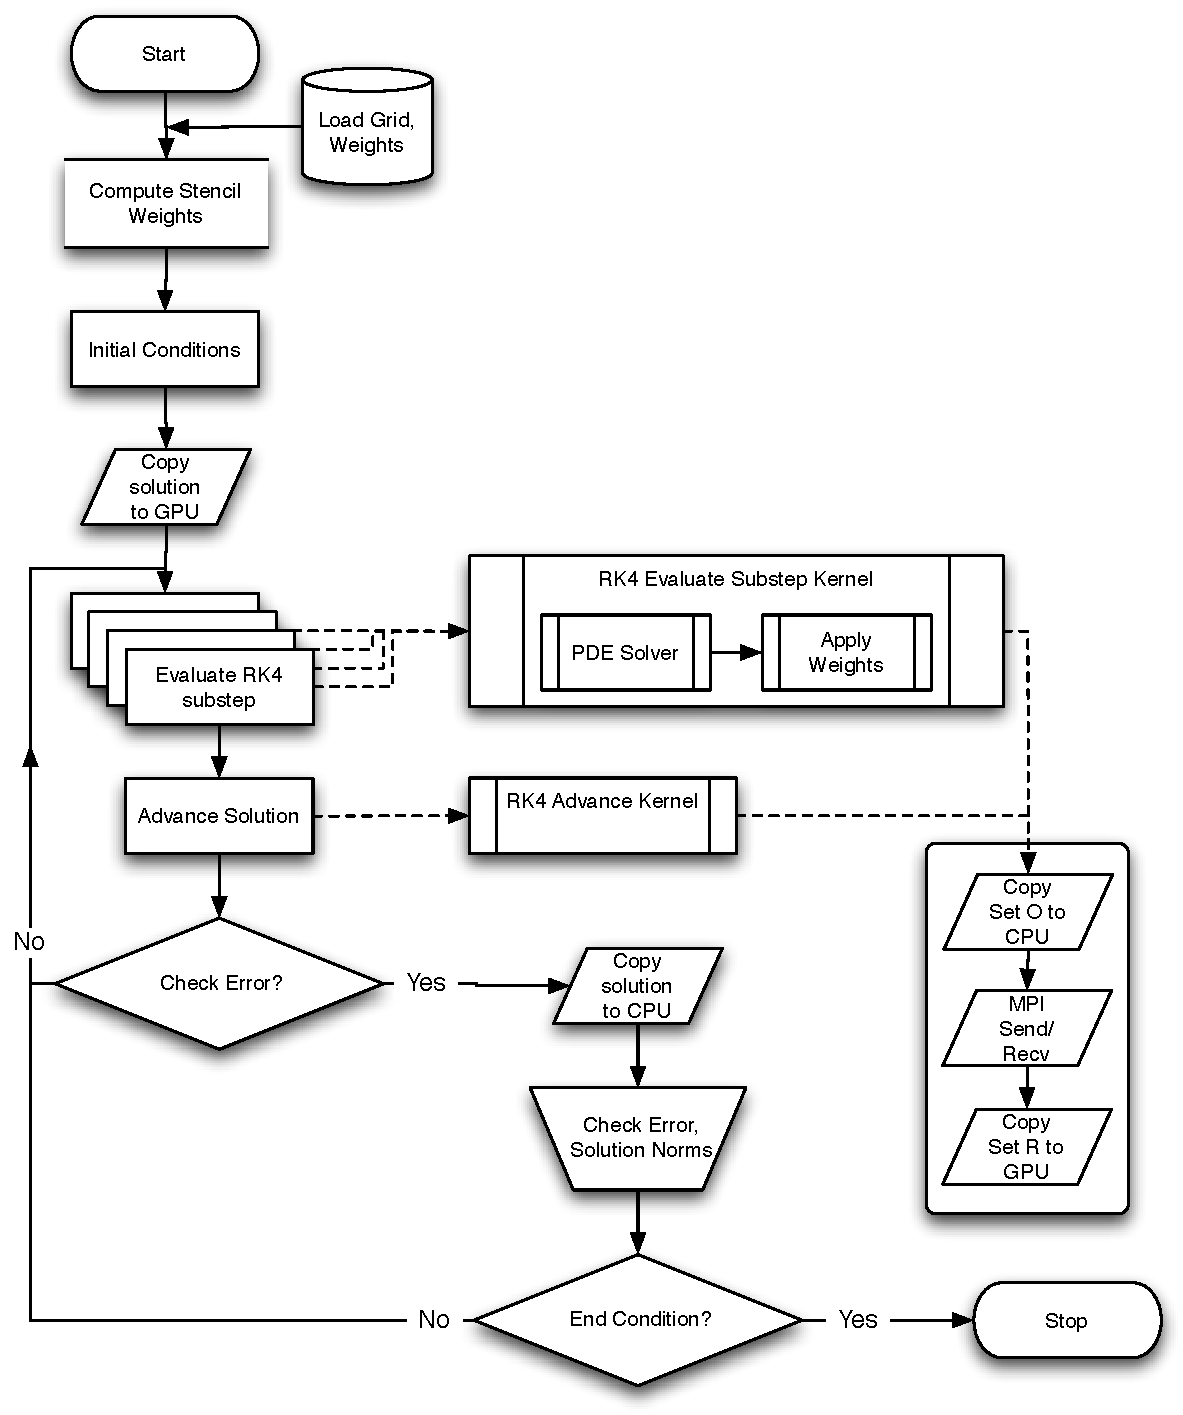
\includegraphics[width=5in]{../figures/paper1/figures/omnigraffle/RK4_multi_GPU_flow.pdf}
      \caption{Workflow for RK4 on multiple GPUs. }
      \label{fig:multi_GPU_flow}
\end{figure}

Figure~\ref{fig:multi_GPU_flow} summarizes the time advancement steps for the multi-CPU/GPU implementation. The RK4 steps are: 
\begin{eqnarray*} 
\mathbf{k}_1 &=& \Delta t f(t_n, \mathbf{u}_n) \\
\mathbf{k}_2 &=& \Delta t f(t_n+\frac{1}{2}\Delta t, \mathbf{u}_n + \frac{1}{2}\mathbf{k}_1) \\
\mathbf{k}_3 &=& \Delta t f(t_n+\frac{1}{2}\Delta t, \mathbf{u}_n + \frac{1}{2}\mathbf{k}_2) \\
\mathbf{k}_4 &=& \Delta t f(t_n+\Delta t, \mathbf{u}_n + \mathbf{k}_3) \\
\mathbf{u}_{n+1} &=& \mathbf{u}_{n} + \frac{1}{6}(\mathbf{k}_1 + 2\mathbf{k}_2 + 2\mathbf{k}_3 +\mathbf{k}_4),
\label{eqn:rk4}
\end{eqnarray*}
where each equation has a corresponding kernel launch. To handle a variety of Runga-Kutta implementations, steps $\mathbf{k}_{1\rightarrow4}$ correspond to calls to the same kernel with different arguments. The evaluation kernel returns two output vectors: 
\begin{enumerate} 
\item $\mathbf{k}_i = \Delta t f(t_n + \alpha_{i} \Delta t, \mathbf{u}_n + \alpha_{i} \mathbf{k}_{i-1})$, for steps $i=1,2,3,4$, and
\item  $\mathbf{u}_n + \alpha_{i+1} \mathbf{k}_i$
\end{enumerate} 
We choose $\alpha_{i}=0, \frac{1}{2}, \frac{1}{2}, 1, 0$ and $\mathbf{k}_{0} = \mathbf{u}_n$. The second output for each $\mathbf{k}_{i=1,2,3}$ serves as input to the next evaluation, $\mathbf{k}_{i+1}$. In an effort to avoid an extra kernel launch---and corresponding memory loads---the SAXPY that produces the second output uses the same evaluation kernel. Both outputs are stored in global device memory. When the computation spans multiple GPUs, steps $\mathbf{k}_{1\rightarrow3}$ are each followed by a communication barrier to synchronize the subsets $\mathcal{O}$ and $\mathcal{R}$ of the second output (this includes copying the subsets between GPU and CPU). An additional synchronization occurs on the updated  solution, $\mathbf{u}_{n+1}$, to ensure that all GPUs share a consistent view of the solution going into the next time-step.

To evaluate $\mathbf{k}_{1\rightarrow4}$, the discretized operators from Equation~(\ref{eq:evaluation_with_hyperviscosity}) are applied using sparse matrix-vector multiplication. If the operator $D$ is composed of multiple derivatives, a differentiation matrix for each derivative is applied independently, including an additional multiplication for the discretized $H$ operator.
 On the GPU, the kernel parallelizes across rows of the DMs, so all derivatives for stencils are computed in one kernel call.


For the GPU, the OpenCL language \cite{OpenCL2009} assumes a lowest common denominator of hardware capabilities to provide functional portability. For example, all target architectures are assumed to support some level of SIMD (Single Instruction Multiple Data) execution for kernels. Multiple \textit{work-items} execute a kernel in parallel. 
A collection of work-items performing the same task is called a \textit{work-group}. While a user might think of work-groups as executing all work-items simultaneously, the work-items are divided at the hardware level into one or more SIMD \textit{warps}, which are executed by a single multiprocessor. On the family of Fermi GPUs, a warp is 32 work-items \cite{CudaGuide2011}. 
OpenCL assumes a tiered memory hierarchy that provides fast but small \textit{local memory} space that is shared within a work-group \cite{OpenCL2009}. Local memory on Fermi GPUs is 48 KB per multiprocessor \cite{CudaGuide2011}. The \textit{global device memory} allows sharing between work-groups and is the slowest but most abundant memory. 
In the GPU computing literature, the terms \textit{thread} and \textit{shared memory} are synonymous to \textit{work-item} and \textit{local memory} respectively, and are preferred below. 

%Although the primary focus of this paper is the implementation 
%and verification of the RBF-FD method across multiple CPUs and GPUs, 
%we have nonetheless tested two approaches to the computation of derivatives 
Our initial implementation of RBF-FD on multiple GPUs (\cite{BolligFlyerErlebacher2012}) tested two approaches to computation of derivatives. 
%assess the potential for further improvements in performance. 
In both cases, the stencil weights are stored in CSR format \cite{Bell2009}, 
a packed one-dimensional array in global memory with all the weights 
of a single stencil in consecutive memory addresses. Each operator is stored as an independent CSR matrix. The consecutive ordering on the weights implies that the solution vector %structured according to the ordering of set $\mathcal{G}$ 
is treated as random access. 

All the computation on the GPU is performed in 8-byte double precision. 


\subsubsection{Naive Approach: One thread per stencil}

In this first implementation, each thread computes 
the derivative at one stencil center  (Figure~\ref{fig:oneThreadPerStencil}). 
The advantage of this approach is trivial concurrency.  Since each stencil has the same number of neighbors, each derivative has an identical number of computations. As long as the number of stencils is a multiple of the warp size, there are no idle threads. Should the total number of stencils be less than a multiple of the warp size, the final warp would contain idle threads, but the impact on efficiency would be minimal assuming the stencil size is sufficiently large. 

Perfect concurrency from a logical point of view does not 
imply perfect efficiency in practice. 
Unfortunately, the naive approach 
is memory bound. When threads access weights in global memory, 
a full warp accesses a 128-byte segment in a single memory operation \cite{CudaGuide2011}.
Since each thread handles a single stencil, the various threads in a warp access data in very disparate areas of global memory, rather than the same segment. This leads to very large slowdowns as extra memory operations are added for each 128-byte segment that the threads of a warp must access.
However, with stencils sharing many common nodes, and the Fermi hardware providing caching, some weights in the unused portions of the segments might remain in cache long enough to hide the cost of so many additional memory loads. 



\begin{figure}[htbp]
      \centering
       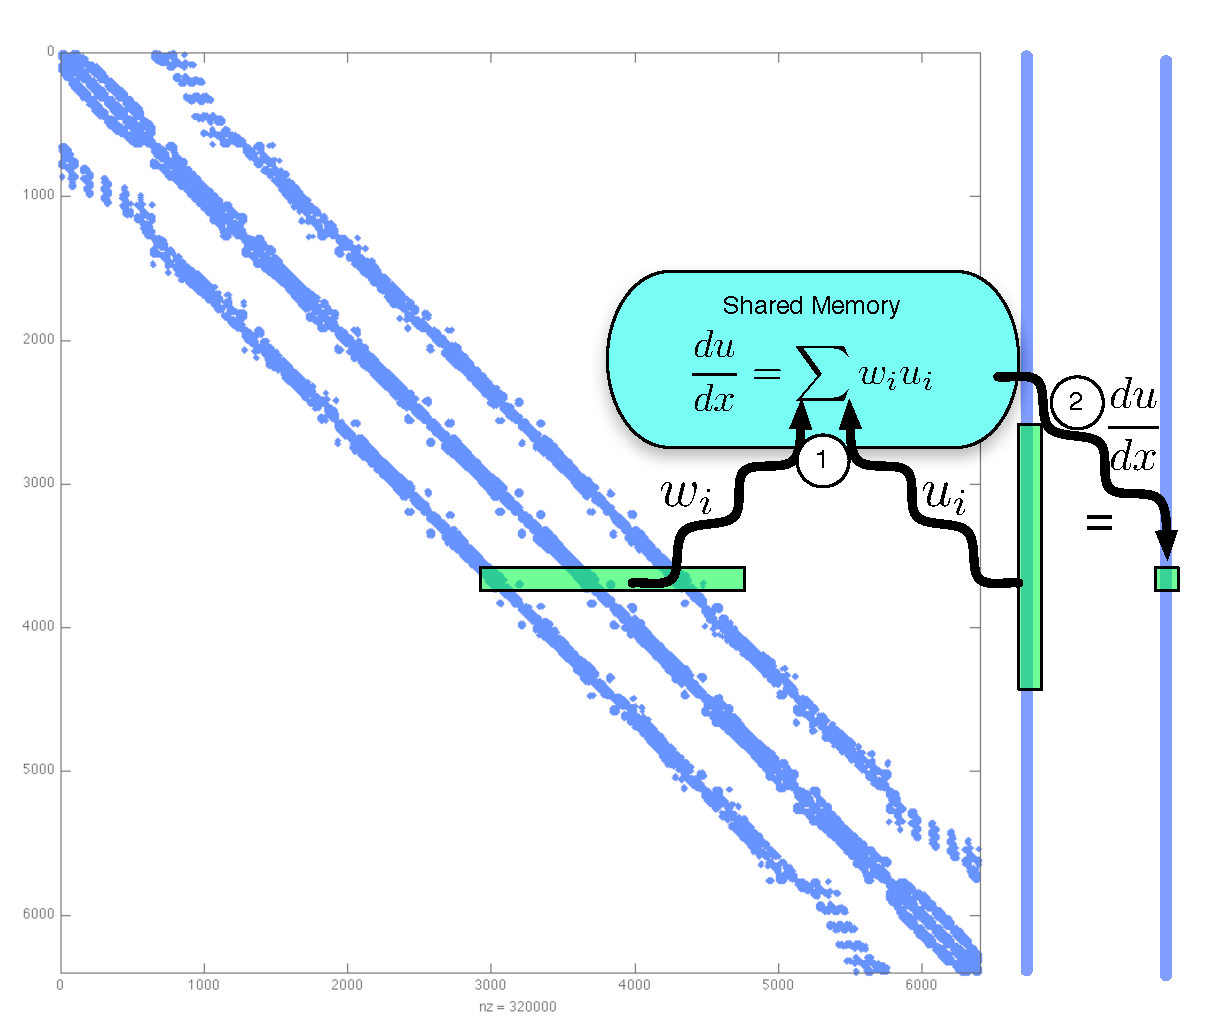
\includegraphics[width=3in]{../figures/paper1/figures/omnigraffle/oneThreadPerStencil.pdf}
      \caption{Naive approach to sparse matrix-vector multiply. Each thread is responsible for the sparse vector dot product of weights and solution values for derivatives at a single stencil.  }
      \label{fig:oneThreadPerStencil}
\end{figure}


\subsubsection{Alternate Approach: One warp per stencil} 

\begin{figure}[htbp]
      \centering
       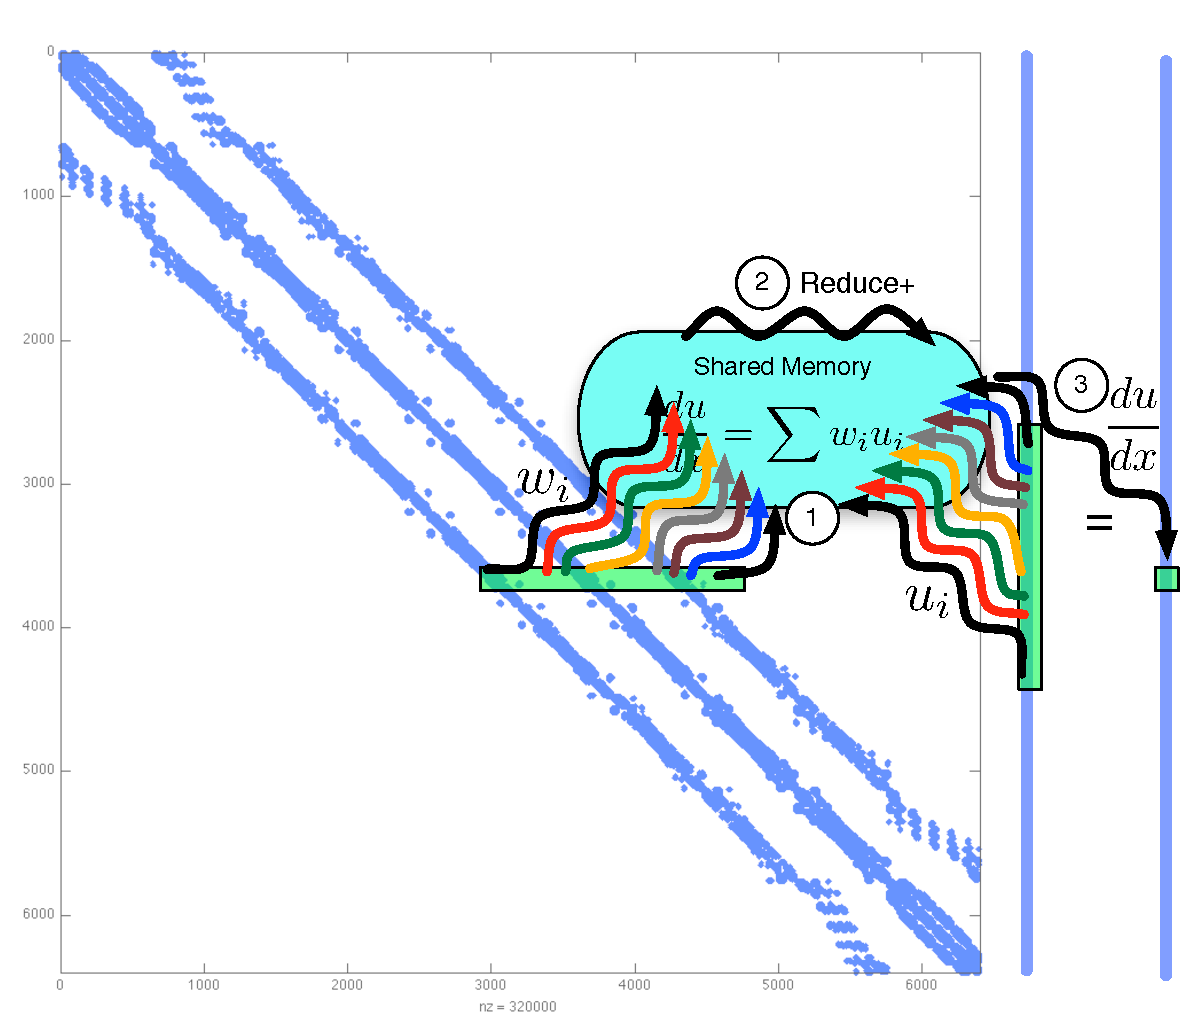
\includegraphics[width=3in]{../figures/paper1/figures/omnigraffle/oneWarpPerStencil.pdf}
      \caption{Alternative approach. A full warp (32 threads) collaborate to apply weights  and compute the derivative at a stencil center. }
      \label{fig:oneWarpPerStencil}
\end{figure}


An alternate approach, illustrated in Figure~\ref{fig:oneWarpPerStencil}, dedicates a full warp of threads to a single stencil. Here, 32 threads load the weights of a stencil and the corresponding elements of the solution vector. As the 32 threads each perform a subset of the dot product, their intermediate sums are accumulated in 32 elements of shared memory (one per thread).
Should  a stencil be larger than the warp size, the warp iterates over the stencil in increments of the warp size until the full dot product is complete. Finally, the first thread of the warp performs a sum reduction across the 32 (warp size)  intermediate sums stored in shared memory and writes the derivative value to global memory. 

By operating on a warp by warp basis, weights for a single stencil are loaded with a reduced number of memory accesses. Memory loads for the solution vector remain random access but see some benefit when solution values for a stencil are in a small neighborhood in the memory space. Proximity in memory can be controlled by node indexing (see e.g., \cite{Bollig2011} and \cite{Connor2009}). 

For stencil sizes smaller than 32, some threads in the warp always remain idle. Idle threads do not slow down the computation within a warp, but under-utilization of the GPU is not desirable. For small stencil sizes, caching on the Fermi can hide some of the cost of memory loads for the naive approach, with no idle threads, making it more efficient. The real strength of one warp per stencil is seen for large stencil sizes. 
As part of future work on optimization, we will consider a parallel reduction in shared memory, as well as assigning multiple stencils to a single warp for small  $n$. 





\subsection{ViennaCL} 

In the time since the publication of \cite{BolligFlyerErlebacher2012} custom OpenCL kernels have been dropped in favor of a library called ViennaCL. 

\begin{figure}
\centering
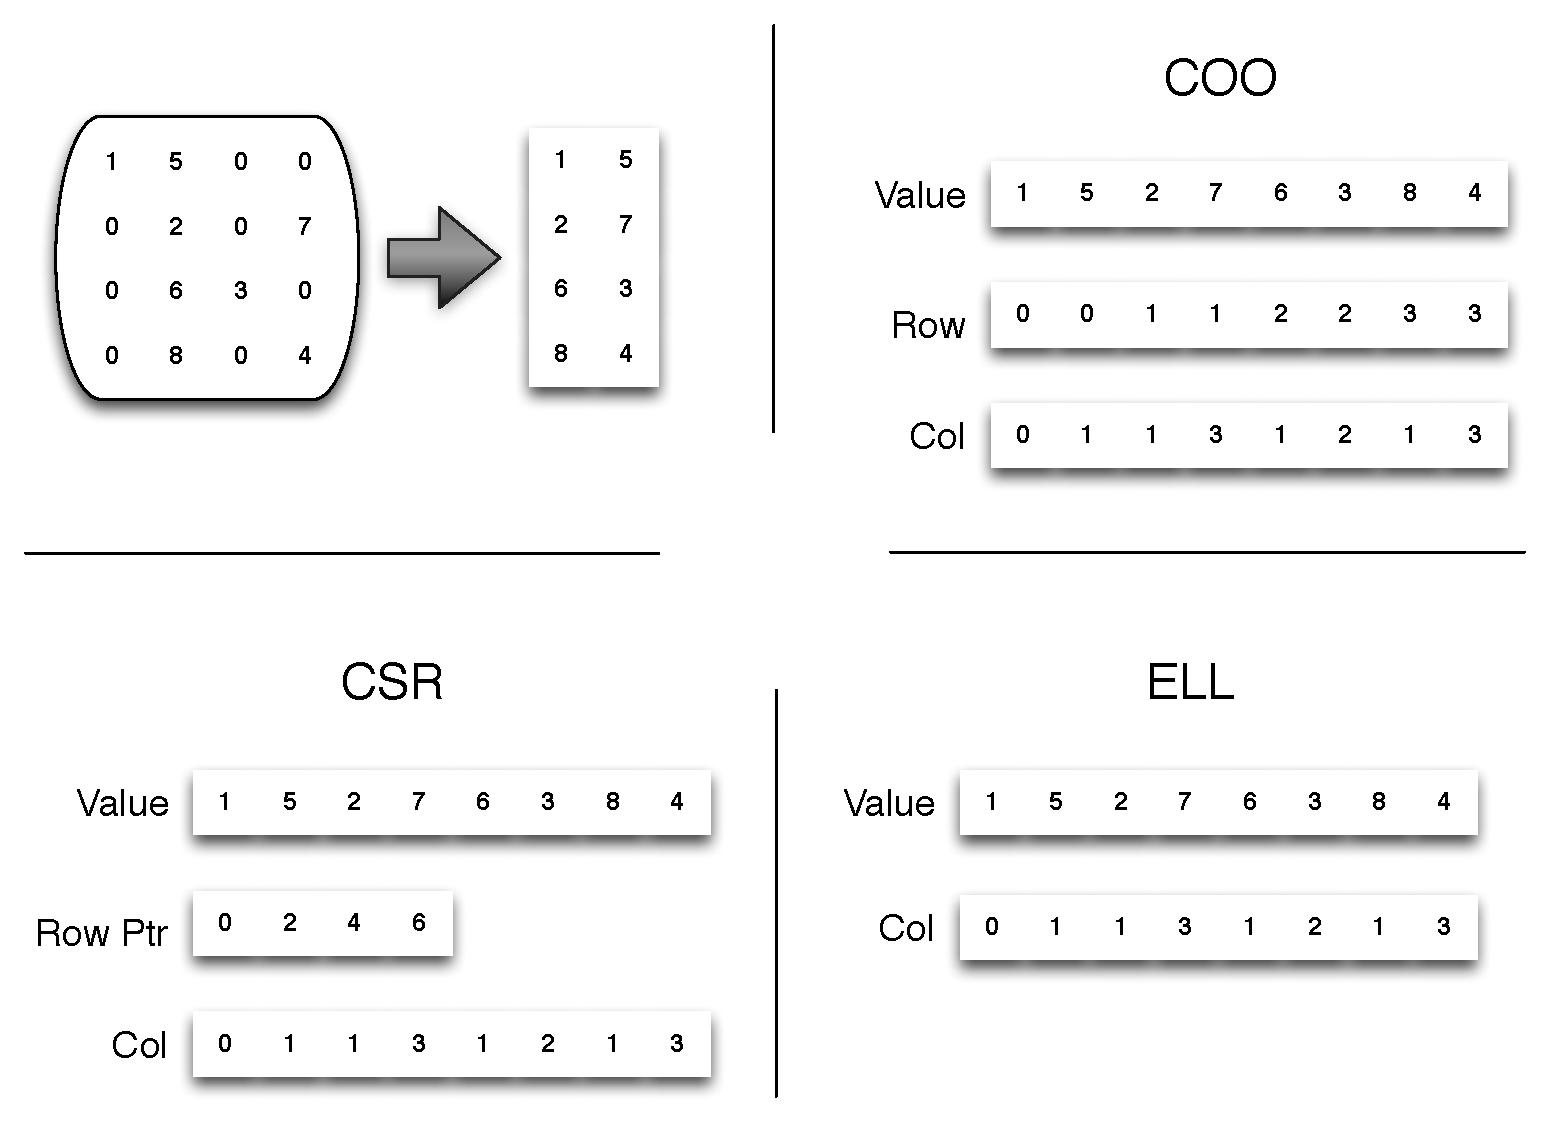
\includegraphics[width=0.9\textwidth]{gpu_content/omnigraffle/SparseStorage.pdf}
\caption{Sparse format example demonstrating a sparse matrix and corresponding storage data structures. ELL format assumes two non-zeros per row. }
\label{fig:sparse_format}
\end{figure}


Other formats exist such as the Hybrid ELL plus CSR (HYB) format \cite{Bell2009}, Diagonal (DIAG) and Jagged Diagonal (JAD) variants, and a number of variants on the ELL format that operate in blocks (BELL), slices (SELL), or both (SBELL) \cite{SuKeutzer2012}. The HYB format stores the bulk of a matrix in an ELL container and the excess non-zeros per row in a CSR format. HYB benefits from reduced storage and memory loads in the ELL, and maintains the generality of a CSR matrix. 





To further optimize RBF-FD on the GPU, we formulate the problem in terms of a Sparse Matrix-Vector Mulitply (SpMV). When we consider the problem in this light we generate a single Differentiation Matrix that can see two optimizations not possible with our stencil-based view: 
\begin{itemize} 
\item First, the sparse containers used in SpMV allow for their own unique optimizations to compress storage and leverage hardware cache.
\item Evaluation of multiple derivatives can be accumulated by association into one matrix operation. This reduces the total number of floating point operations required per iteration. 
\end{itemize}


%TODO: tell the story of ViennaCL. 
%TODO: what motivated the switch
The library includes a variety of sparse matrix formats, solvers, preconditioners, etc. Dense and sparse containers simplify targeting the GPU. 

At the onset of work with ViennaCL two things were apparent: 1) the library was incredibly powerful but limited to square matrices; and 2) the library had no support for distributed computing. Our implementation of RBF-FD (\cite{BolligRBFFDGPU}) required rectangular matrices resulting from domain decomposition. The enhancements to the API have since been added to the main branch of ViennaCL. 


CSR Bytes:Flop ratio: \url{http://arxiv.org/pdf/1101.0091v1.pdf}





%TODO: list example loops for sparse kernels

\section{Performance Comparison}
\subsection{Performance of Cosine CL vs VCL}
\subsection{VCL Formats Comparison}

Our assumption with RBF-FD in this manuscript is that all stencils will have equal size. Due to this, the ELL format is preferred as the default. 
 


\subsection{Intel Phi} 

As part of future work into accelerating RBF methods, investigations are underway into the new Intel Phi architecture. The variety of hardware available on Cascade will help us establish a clear argument in the choice of accelerator type and resolve the dilemma between choosing Phi vs GPU for our method. Since RBFs generalize other methods, our results should have broad reaching impact to answer similar questions for related methods.

%TODO: preliminary benchmarks on performance of ViennaCL SpMV. 

With the generalization of RBF-FD derivative computation formulated as a sparse matrix multiplication, we can 
% TODO: mention CUSP as alternative but concentrate on VCL
consider the various sparse formats provided by CUSP and ViennaCL. 

%TODO later: \item All stencils with non-uniform size
%TODO: What is the optimal choice of sparse container? How do the sparse containers compare in performance to each other, and to our custom kernels? What can we conclude? 



\section{GPU SpMV Performance}

This section presents benchmarks obtained on a variety of GPU hardware. 

Data from Keeneland

Data from Cascade

Data from 




\section{Conclusions and Future Work}

Conclude: sparse containers allow increased efficiency compared to our custom kernels. The custom kernels compete with CSR and COO. 




We compare the performance of our custom kernel to ViennaCL kernels (ELL, CSR, COO), UBlas (CSR) 


ViennaCL allows control of the number of work-items for each kernel. 

The library can tune itself to find the optimal number of work-items based on the device. 

%TODO: what is profile for each GPU type
%TODO: What is the significance of tuning on our problem $n=17, 31, 50, 101,$ etc. 
%TODO: experiment: SpMV on N=10^6, n = variable (5->105)
%TODO: idealized experiment: SpMV on N=10^6 regular grid with n=variable.




%TODO: finish fill-in
When matrix is sparse, a direct LU decomposition causes fill-in on factorization. In some cases the fill-in can be minimal, but in general one must assume that fill in can turn the sparse matrix into a dense matrix. To invert and solve Equation~\ref{eq:implicit_eq}, use an iterative solver like GMRES. The GMRES algorithm (described further in Chapter~\ref{chap:applications} applies successive SpMVs along with other vector operations to converge on a solution. Due to the dominance of SpMV in GMRES, the performance of RBF-FD reduces once again to SpMV.





%
%
%Hardware architecture
%•	Memory layout
%•	Processing cores
%•	Trends in hardware since 2006 (additions and benfits)
%Optimization
%•	SpMV memory layout
%•	Scheduling threads
%•	Reductions
%OpenCL
%•	Why? 
%o	Cross platform support
%o	Asynchronous Queuing with Dependencies
%•	Implementations details
%o	Kernel
%o	Work-Item
%o	Work-Group
%o	NDRange
%o	Queue
%o	Etc.
%•	How does it compare to CUDA? Phi
%•	Latest trends
%o	Phi: bind against MKL for optimized CPU and MIC
%o	CUDA-MPI
%o	CUDA Sub-Kernel calls
%o	CUDA uptake 
%•	E.g., Matlab (MEX compiled kernel wrappers)
%Conclusions on GPGPU
%•	Benefits are good
%o	Cheap to purchase < $1K
%o	superior performance 1.2 TFLOPs possible in one card
%o	was a trending technology (major uptake in supercomputing and national labs)
%•	Downsides were varied
%•	Overall Impression is that
%o	Uptake was wide-spread for research projects
%o	Focus was on determining limits of the hardware
%•	Many studies focused on optimization of primitives which allow general use in applications such as RBF-FD without recreating the wheel when it comes to optimal algorithms. Allows researchers to concentrate on other investigations into application, preconditioning, data analysis, etc.
%Newcomers to the field are interested USING gpgpu applications, rather than writing them  




\ifstandalone
\bibliographystyle{plain}
\bibliography{merged_references}
\end{document}
\else
\expandafter\endinput
\fi


